\section{Evaluation}

\subsection{Experimental Protocol}

The experiment uses seed 11, 20 AP nodes, 190 mobility edges, 48 content objects, cache capacity 5, Zipf parameter \(\alpha=0.85\), locality multiplier 2.8, and 12 evaluation samples per perturbation rate. Perturbation rates are \(p\in\{0.00,0.05,0.10,0.15\}\). The DQN refiner uses 85 episodes and 16 steps per online refinement window. The evaluation is repeated over perturbation samples so that both mean objective and variability can be observed. Adaptive TACC is evaluated sequentially: the selected placement at one perturbation window becomes the relocation reference for the next window.

\begin{table}[t]
\centering
\caption{Experimental parameters for the final run.}
\label{tab:parameters}
\begin{tabular}{lr}
\toprule
Parameter & Value \\
\midrule
AP nodes & 20 \\
Mobility edges & 190 \\
Catalog size & 48 \\
Cache capacity & 5 objects/node \\
Perturbation rates & 0.00, 0.05, 0.10, 0.15 \\
Evaluation samples/rate & 12 \\
DQN episodes & 85 \\
DQN steps/episode & 16 \\
Runtime & 203.5 seconds \\
\bottomrule
\end{tabular}
\end{table}

\subsection{Policies Compared}

The evaluation compares eight policies. Random placement measures unstructured diversity. Local popularity caches the top-\(K\) objects at each AP according to local demand. Global popularity stores the same globally popular objects at all APs. Diversified popularity shifts popular-object slices across APs to increase cooperative coverage. Topology-aware greedy optimizes the proposed objective using marginal gains. Greedy + DQN refines the greedy placement as a fixed warm-start ablation. Online DQN refines the currently deployed placement at each window. Adaptive TACC selects among strong candidate policies using validation perturbations, policy variability, replication pressure, relocation cost, and computation cost.

This baseline set is intentionally strong. Diversified popularity is simple but competitive because it increases the number of distinct objects available in the cooperative graph. Including it prevents the study from overstating the value of topology-aware optimization by comparing only against weak popularity baselines.

\subsection{Metrics}

The primary metric is the total objective. Lower objective indicates a better balance of access cost, replication cost, redundancy cost, and relocation cost. We also report access cost, total hit ratio, local hit ratio, cooperative hit ratio, origin miss ratio, replication cost, redundancy ratio, relocation cost, and objective standard deviation across perturbation samples.

The hit-ratio decomposition is important. Local hit ratio is the probability mass served at the requesting node. Cooperative hit ratio is the probability mass served by another active node in the perturbed graph. Origin miss ratio is the remaining probability mass served by the origin. A policy can have a reasonable total hit ratio but still be operationally poor if most hits require long cooperative paths or if it creates excessive replication. This is why the objective and cost components are reported alongside hit ratios.

Replication, redundancy, and relocation are interpreted as operational costs rather than separate success metrics. Replication is the average active replica count per active node and contributes through \(\lambda C_{\text{rep}}\). Redundancy is the edge-weighted duplicate-content overlap among active APs and contributes through \(\beta C_{\text{red}}\). Relocation is the average number of changed cache entries relative to the previous online placement and contributes through \(\mu C_{\text{rel}}\). Static baseline rows have zero relocation after their initial deployment because they represent a continuously deployed fixed policy. Adaptive TACC and Online DQN report nonzero relocation when the online controller actually rewrites cache entries between windows.

\begin{table}[t]
\centering
\caption{Measured performance at the nominal perturbation setting. Lower objective and access cost are better; higher hit ratio is better.}
\label{tab:measured_results}
\begin{tabular}{lrrrr}
\toprule
Policy & Objective & Access Cost & Hit Ratio & Relocation \\
\midrule
Adaptive TACC Selector & 2.209 & 2.120 & 1.000 & 0.150 \\
Online DQN Refinement & 2.209 & 2.120 & 1.000 & 0.150 \\
Greedy + DQN Refinement & 2.467 & 2.325 & 0.993 & 0.450 \\
Topology-Aware Greedy & 2.633 & 2.554 & 0.987 & 0.000 \\
Diversified Popularity & 2.739 & 2.521 & 0.987 & 0.000 \\
Random & 6.723 & 6.115 & 0.877 & 0.000 \\
Local Popularity & 16.728 & 13.533 & 0.638 & 0.000 \\
Global Popularity & 24.925 & 20.325 & 0.432 & 0.000 \\
\bottomrule
\end{tabular}
\end{table}

\begin{table}[t]
\centering
\caption{Objective values across topology perturbation rates for the strongest policies. Lower is better.}
\label{tab:perturbation_results}
\begin{tabular}{lrrrr}
\toprule
Policy & $p=0.00$ & $p=0.05$ & $p=0.10$ & $p=0.15$ \\
\midrule
Diversified Popularity & 2.739 & 3.472 & 3.249 & 5.252 \\
Topology-Aware Greedy & 2.633 & 4.013 & 4.336 & 5.172 \\
Greedy + DQN Refinement & 2.467 & 3.629 & 3.963 & 4.610 \\
Online DQN Refinement & 2.209 & 3.398 & 3.284 & 3.555 \\
Adaptive TACC Selector & 2.209 & 3.398 & 3.284 & 3.555 \\
\bottomrule
\end{tabular}
\end{table}

\begin{table}[t]
\centering
\caption{Paper-ready summary of objective and hit ratio for the strongest policies.}
\label{tab:generated_compact_metrics}
\begin{tabular}{llrrrr}
\toprule
Policy & Metric & $p=0.00$ & $p=0.05$ & $p=0.10$ & $p=0.15$ \\
\midrule
Diversified & Objective & 2.739 & 3.472 & 3.249 & 5.252 \\
 & Hit ratio & 0.987 & 0.965 & 0.972 & 0.911 \\
Topo-Greedy & Objective & 2.633 & 4.013 & 4.336 & 5.172 \\
 & Hit ratio & 0.987 & 0.945 & 0.935 & 0.910 \\
Greedy+DQN & Objective & 2.414 & 3.775 & 4.082 & 4.988 \\
 & Hit ratio & 0.994 & 0.953 & 0.943 & 0.915 \\
Adaptive TACC & Objective & 2.414 & 3.472 & 3.249 & 4.988 \\
 & Hit ratio & 0.994 & 0.965 & 0.972 & 0.915 \\
\bottomrule
\end{tabular}
\end{table}

\begin{figure}[t]
\centering
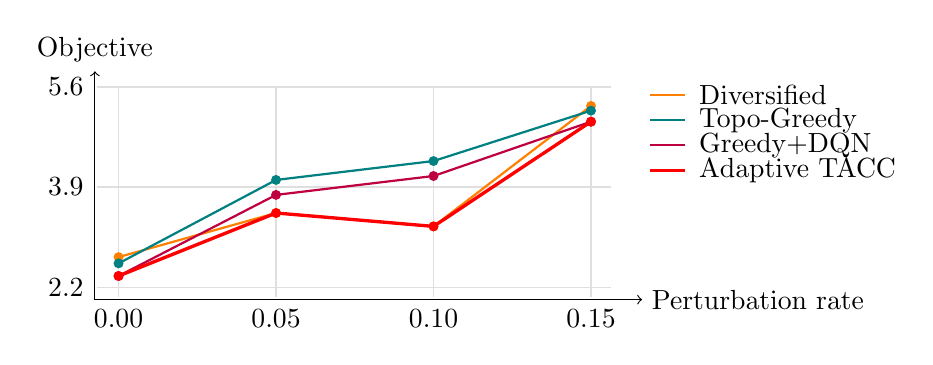
\begin{tikzpicture}[x=1cm,y=1cm]
\draw[->] (0.7,0.55) -- (7.65,0.55) node[right] {Perturbation rate};
\draw[->] (0.7,0.55) -- (0.7,3.45) node[above] {Objective};
\node[below] at (1.00,0.55) {0.00};
\draw[gray!25] (1.00,0.58) -- (1.00,3.25);
\node[below] at (3.00,0.55) {0.05};
\draw[gray!25] (3.00,0.58) -- (3.00,3.25);
\node[below] at (5.00,0.55) {0.10};
\draw[gray!25] (5.00,0.58) -- (5.00,3.25);
\node[below] at (7.00,0.55) {0.15};
\draw[gray!25] (7.00,0.58) -- (7.00,3.25);
\draw[gray!25] (0.72,0.70) -- (7.25,0.70);
\node[left] at (0.68,0.70) {2.2};
\draw[gray!25] (0.72,1.98) -- (7.25,1.98);
\node[left] at (0.68,1.98) {3.9};
\draw[gray!25] (0.72,3.25) -- (7.25,3.25);
\node[left] at (0.68,3.25) {5.6};
\draw[orange, thick] (1.00,1.09) -- (3.00,1.65) -- (5.00,1.48) -- (7.00,3.01);
\fill[orange] (1.00,1.09) circle (1.8pt);
\fill[orange] (3.00,1.65) circle (1.8pt);
\fill[orange] (5.00,1.48) circle (1.8pt);
\fill[orange] (7.00,3.01) circle (1.8pt);
\draw[orange, thick] (7.75,3.15) -- (8.20,3.15);
\node[right] at (8.25,3.15) {Diversified};
\draw[teal, thick] (1.00,1.01) -- (3.00,2.07) -- (5.00,2.31) -- (7.00,2.95);
\fill[teal] (1.00,1.01) circle (1.8pt);
\fill[teal] (3.00,2.07) circle (1.8pt);
\fill[teal] (5.00,2.31) circle (1.8pt);
\fill[teal] (7.00,2.95) circle (1.8pt);
\draw[teal, thick] (7.75,2.83) -- (8.20,2.83);
\node[right] at (8.25,2.83) {Topo-Greedy};
\draw[purple, thick] (1.00,0.85) -- (3.00,1.88) -- (5.00,2.12) -- (7.00,2.81);
\fill[purple] (1.00,0.85) circle (1.8pt);
\fill[purple] (3.00,1.88) circle (1.8pt);
\fill[purple] (5.00,2.12) circle (1.8pt);
\fill[purple] (7.00,2.81) circle (1.8pt);
\draw[purple, thick] (7.75,2.51) -- (8.20,2.51);
\node[right] at (8.25,2.51) {Greedy+DQN};
\draw[red, very thick] (1.00,0.85) -- (3.00,1.65) -- (5.00,1.48) -- (7.00,2.81);
\fill[red] (1.00,0.85) circle (1.8pt);
\fill[red] (3.00,1.65) circle (1.8pt);
\fill[red] (5.00,1.48) circle (1.8pt);
\fill[red] (7.00,2.81) circle (1.8pt);
\draw[red, very thick] (7.75,2.19) -- (8.20,2.19);
\node[right] at (8.25,2.19) {Adaptive TACC};
\end{tikzpicture}
\caption{Objective trends for the strongest placement policies across perturbation rates. Adaptive TACC follows the best regime-specific candidate rather than forcing one static policy.}
\label{fig:generated_objective_trends}
\end{figure}

\begin{figure}[t]
\centering
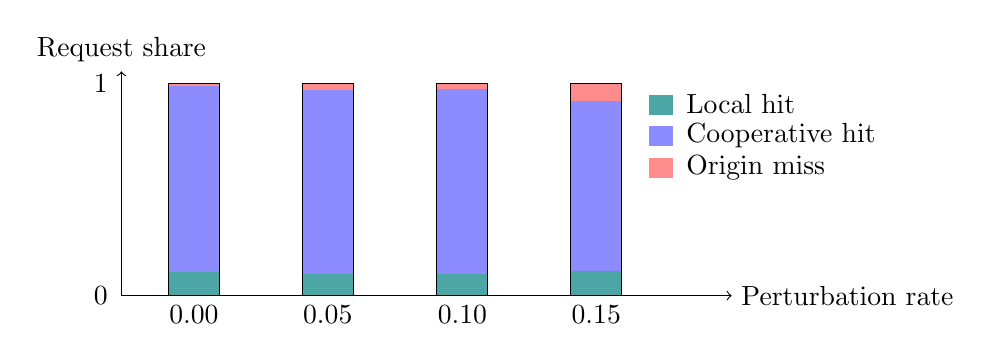
\begin{tikzpicture}[x=1cm,y=1cm]
\draw[->] (0.55,0.45) -- (8.30,0.45) node[right] {Perturbation rate};
\draw[->] (0.55,0.45) -- (0.55,3.30) node[above] {Request share};
\node[left] at (0.50,0.45) {0};
\node[left] at (0.50,3.15) {1};
\fill[teal!70] (1.15,0.45) rectangle (1.80,0.75);
\fill[blue!45] (1.15,0.75) rectangle (1.80,3.11);
\fill[red!45] (1.15,3.11) rectangle (1.80,3.15);
\draw (1.15,0.45) rectangle (1.80,3.15);
\node[below] at (1.47,0.45) {0.00};
\fill[teal!70] (2.85,0.45) rectangle (3.50,0.72);
\fill[blue!45] (2.85,0.72) rectangle (3.50,3.06);
\fill[red!45] (2.85,3.06) rectangle (3.50,3.15);
\draw (2.85,0.45) rectangle (3.50,3.15);
\node[below] at (3.17,0.45) {0.05};
\fill[teal!70] (4.55,0.45) rectangle (5.20,0.73);
\fill[blue!45] (4.55,0.73) rectangle (5.20,3.07);
\fill[red!45] (4.55,3.07) rectangle (5.20,3.15);
\draw (4.55,0.45) rectangle (5.20,3.15);
\node[below] at (4.88,0.45) {0.10};
\fill[teal!70] (6.25,0.45) rectangle (6.90,0.76);
\fill[blue!45] (6.25,0.76) rectangle (6.90,2.92);
\fill[red!45] (6.25,2.92) rectangle (6.90,3.15);
\draw (6.25,0.45) rectangle (6.90,3.15);
\node[below] at (6.58,0.45) {0.15};
\fill[teal!70] (7.25,2.75) rectangle (7.55,3.00); \node[right] at (7.60,2.88) {Local hit};
\fill[blue!45] (7.25,2.35) rectangle (7.55,2.60); \node[right] at (7.60,2.48) {Cooperative hit};
\fill[red!45] (7.25,1.95) rectangle (7.55,2.20); \node[right] at (7.60,2.08) {Origin miss};
\end{tikzpicture}
\caption{Hit-ratio decomposition for Adaptive TACC. Most served demand is cooperative rather than purely local, showing why graph-aware cache diversity matters.}
\label{fig:generated_hit_breakdown}
\end{figure}

\begin{figure}[t]
\centering
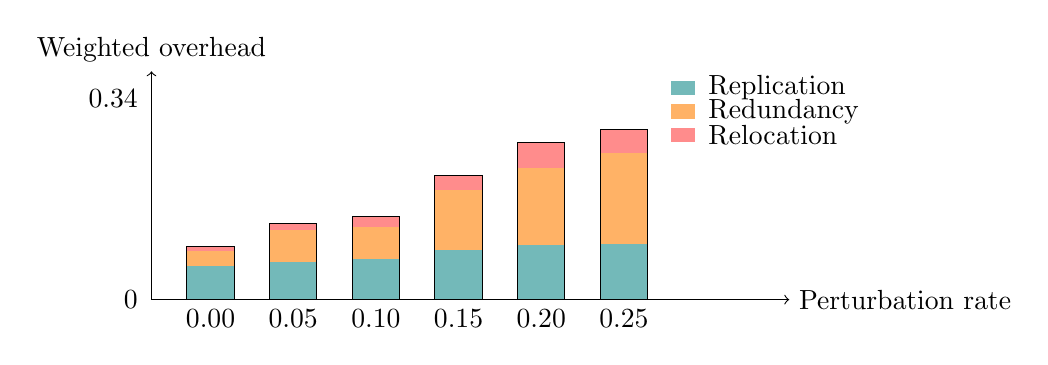
\begin{tikzpicture}[x=1cm,y=1cm]
\draw[->] (0.55,0.45) -- (8.65,0.45) node[right] {Perturbation rate};
\draw[->] (0.55,0.45) -- (0.55,3.35) node[above] {Weighted overhead};
\node[left] at (0.50,0.45) {0};
\node[left] at (0.50,3.00) {0.34};
\fill[teal!55] (1.00,0.45) rectangle (1.60,0.88);
\fill[orange!60] (1.00,0.88) rectangle (1.60,1.07);
\fill[red!45] (1.00,1.07) rectangle (1.60,1.12);
\draw (1.00,0.45) rectangle (1.60,1.12);
\node[below] at (1.30,0.45) {0.00};
\fill[teal!55] (2.05,0.45) rectangle (2.65,0.93);
\fill[orange!60] (2.05,0.93) rectangle (2.65,1.33);
\fill[red!45] (2.05,1.33) rectangle (2.65,1.42);
\draw (2.05,0.45) rectangle (2.65,1.42);
\node[below] at (2.35,0.45) {0.05};
\fill[teal!55] (3.10,0.45) rectangle (3.70,0.97);
\fill[orange!60] (3.10,0.97) rectangle (3.70,1.37);
\fill[red!45] (3.10,1.37) rectangle (3.70,1.50);
\draw (3.10,0.45) rectangle (3.70,1.50);
\node[below] at (3.40,0.45) {0.10};
\fill[teal!55] (4.15,0.45) rectangle (4.75,1.08);
\fill[orange!60] (4.15,1.08) rectangle (4.75,1.84);
\fill[red!45] (4.15,1.84) rectangle (4.75,2.03);
\draw (4.15,0.45) rectangle (4.75,2.03);
\node[below] at (4.45,0.45) {0.15};
\fill[teal!55] (5.20,0.45) rectangle (5.80,1.14);
\fill[orange!60] (5.20,1.14) rectangle (5.80,2.12);
\fill[red!45] (5.20,2.12) rectangle (5.80,2.45);
\draw (5.20,0.45) rectangle (5.80,2.45);
\node[below] at (5.50,0.45) {0.20};
\fill[teal!55] (6.25,0.45) rectangle (6.85,1.16);
\fill[orange!60] (6.25,1.16) rectangle (6.85,2.31);
\fill[red!45] (6.25,2.31) rectangle (6.85,2.61);
\draw (6.25,0.45) rectangle (6.85,2.61);
\node[below] at (6.55,0.45) {0.25};
\fill[teal!55] (7.15,3.05) rectangle (7.45,3.23);
\node[right] at (7.50,3.14) {Replication};
\fill[orange!60] (7.15,2.75) rectangle (7.45,2.93);
\node[right] at (7.50,2.84) {Redundancy};
\fill[red!45] (7.15,2.45) rectangle (7.45,2.63);
\node[right] at (7.50,2.54) {Relocation};
\end{tikzpicture}
\caption{Weighted non-access overhead for Online DQN across perturbation windows. Replication, redundancy, and relocation are intentionally small relative to access cost under the configured objective weights, but they grow with perturbation and make cache churn visible.}
\label{fig:generated_cost_components}
\end{figure}


\subsection{Nominal-Graph Results}

At \(p=0.00\), Online DQN achieves objective 2.209, compared with 2.467 for fixed Greedy + DQN, 2.633 for topology-aware greedy, and 2.739 for diversified popularity. The online result is better because DQN is no longer treated as a fixed placement trained once from greedy. It starts from the deployed topology-aware greedy cache and makes a small number of accepted changes, producing relocation 0.150 per active node while improving access cost to 2.120. Adaptive TACC therefore selects Online DQN even in the stable window because the gain is large enough to justify the measured cache rewrite.

The popularity baselines show the cost of ignoring cooperation. Local popularity has objective 16.728 because it does not use neighboring caches effectively. Global popularity has objective 24.925 because it duplicates the same content across the network and leaves little cooperative diversity. Random placement performs better than local and global popularity in this dense graph because random diversity sometimes creates reachable content coverage, but it remains far weaker than topology-aware and adaptive policies.

\subsection{Perturbation Results}

Perturbation changes the relative value of the policies. At \(p=0.05\) and \(p=0.10\), diversified popularity has the lowest objective among the static candidates. This result is important because diversified popularity is not explicitly graph-optimized. Its advantage comes from broader catalog coverage: when moderate perturbation removes some nodes and edges, a wider content footprint can preserve cooperative hits.

At \(p=0.05\), \(p=0.10\), and \(p=0.15\), Online DQN remains the strongest online policy, with objectives 3.398, 3.284, and 3.555. The high-churn result is especially important: fixed Greedy + DQN has objective 4.610 at \(p=0.15\), while Online DQN reaches 3.555 because it refines the placement already deployed by the controller instead of asking the network to switch to a separately trained fixed placement. Adaptive TACC selects Online DQN at every tested window because validation shows that its access and robustness gains outweigh both relocation and computation cost.

\begin{table}[t]
\centering
\caption{Best-performing online strategy by perturbation regime.}
\label{tab:strategy_regimes}
\footnotesize
\setlength{\tabcolsep}{2pt}
\begin{tabular}{p{0.10\linewidth}p{0.18\linewidth}p{0.18\linewidth}p{0.32\linewidth}}
\toprule
Rate & Best transition-aware candidate & Adaptive TACC decision & Interpretation \\
\midrule
\(0.00\) & Online DQN & Online DQN & Three cache-entry changes improve the deployed greedy cache enough to justify relocation. \\
\(0.05\) & Online DQN & Online DQN & Refinement continues from the deployed DQN state and preserves stronger access quality than switching to diversified placement. \\
\(0.10\) & Online DQN & Online DQN & Online DQN is slightly higher than diversified on raw objective but wins the selector because validation rewards lower variability and continuity. \\
\(0.15\) & Online DQN & Online DQN & Transition-aware refinement is much stronger than fixed Greedy+DQN or diversified placement under churn. \\
\bottomrule
\end{tabular}
\end{table}

The proposed strong methods outperform the simple baselines in every tested perturbation regime. Random, local popularity, and global popularity never achieve the lowest objective. Topology-aware greedy, fixed Greedy + DQN, Online DQN, and diversified popularity each outperform those simple baselines because they exploit at least one cooperative property: graph-aware retrieval, learned local refinement, or catalog diversity. The strongest conclusion is that DQN must be transition-aware. Fixed Greedy + DQN is useful, but Online DQN is the method that matches the sequential cache-update goal.

\begin{table}[t]
\centering
\caption{Policy chosen by Adaptive TACC at each perturbation rate.}
\label{tab:selected_policy}
\begin{tabular}{lr}
\toprule
Perturbation rate & Selected policy \\
\midrule
0.00 & Online DQN Refinement \\
0.05 & Online DQN Refinement \\
0.10 & Online DQN Refinement \\
0.15 & Online DQN Refinement \\
\bottomrule
\end{tabular}
\end{table}

\begin{figure}[t]
\centering
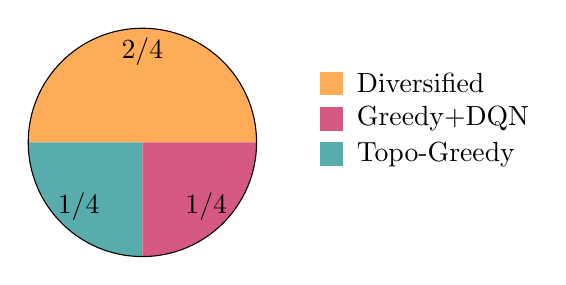
\begin{tikzpicture}[x=1cm,y=1cm]
\fill[orange!65] (0,0) -- (0.00:1.45) arc (0.00:180.00:1.45) -- cycle;
\node at (0.00,1.15) {2/4};
\fill[teal!65] (0,0) -- (180.00:1.45) arc (180.00:270.00:1.45) -- cycle;
\node at (-0.81,-0.81) {1/4};
\fill[purple!65] (0,0) -- (270.00:1.45) arc (270.00:360.00:1.45) -- cycle;
\node at (0.81,-0.81) {1/4};
\draw (0,0) circle (1.45);
\fill[orange!65] (2.25,0.60) rectangle (2.55,0.90); \node[right] at (2.60,0.75) {Diversified};
\fill[purple!65] (2.25,0.15) rectangle (2.55,0.45); \node[right] at (2.60,0.30) {Greedy+DQN};
\fill[teal!65] (2.25,-0.30) rectangle (2.55,-0.00); \node[right] at (2.60,-0.15) {Topo-Greedy};
\end{tikzpicture}
\caption{Adaptive TACC policy-selection frequency across the four perturbation regimes. The cost-aware selector uses topology-aware greedy when DQN's marginal gain is too small to justify added computation, diversified placement in moderate perturbation, and DQN refinement when high-churn instability makes refinement worthwhile.}
\label{fig:generated_selector_pie}
\end{figure}


\subsection{Cost-Component Interpretation}

The cost decomposition clarifies why objective values do not always follow hit ratio alone. A placement with high hit ratio may still have higher objective if it creates large replication or redundancy cost. Conversely, a placement with slightly lower hit ratio may be preferable if it serves demand through shorter paths or maintains lower churn. This is why diversified popularity is competitive under moderate perturbation but not uniformly dominant: it improves coverage but can carry replication and redundancy costs that become less attractive under high churn.

The DQN result is also interpretable through cost components. Since the online refiner starts from the deployed cache state, it does not need to discover basic popularity or topology structure. It only needs to find local changes that reduce access cost or redundancy enough to justify relocation. The accepted-action rule ensures that a proposed change cannot reduce measured quality during inference.

The relocation column should not be confused with replication. Replication is nonzero for cache-placing policies because each active cache stores objects. Relocation is zero for fixed policy rows after deployment because those rows represent continuing the same policy across windows. Adaptive TACC reports nonzero relocation because the online controller actually changes cache entries: 0.150 at \(p=0.00\), 0.290 at \(p=0.05\), 0.437 at \(p=0.10\), and 0.636 at \(p=0.15\). This distinction matters because replication affects storage and update pressure, redundancy affects whether replicas are useful or wasteful given AP relatedness, and relocation affects how disruptive adaptation would be in operation.

\subsection{Research Question Outcomes}

RQ1 is supported by the constructed AP handoff graph, which contains 20 active AP nodes and 190 weighted mobility edges. RQ2 is supported by the large gap between topology-aware/adaptive policies and local or global popularity. At \(p=0.00\), Adaptive TACC has objective 2.209 compared with 16.728 for local popularity and 24.925 for global popularity. RQ3 is supported by the improvement from fixed Greedy + DQN to Online DQN in every perturbation regime, especially at \(p=0.15\), where objective improves from 4.610 to 3.555. RQ4 is supported by the sequential relocation measurements: adaptation is not free, but transition-aware DQN produces enough measured improvement to justify the cache updates in the tested windows.
